\documentclass[aspectratio=169]{beamer}
\usepackage{hyperref}
\hypersetup{
	pdfstartpage=1 ,
	pdfpagemode=FullScreen % Start in full-screen mode
	% Ensure it starts from page 1
}
\usetheme{CambridgeUS}
\usecolortheme{beaver}
\useoutertheme[subsection=false]{smoothbars}
\usepackage{graphicx}
\usepackage{dirtytalk}
\usepackage{pgf}
\graphicspath{{img}}
\usepackage{siunitx}
\usepackage{multicol}
\usepackage{multimedia}
\usepackage{minted}
\usepackage{subcaption}
\usepackage{braket}
\setcounter{MaxMatrixCols}{11}
\setbeamertemplate{navigation symbols}{}

\setminted{fontsize=\scriptsize, tabsize=2}

\captionsetup{font=footnotesize}

\newcounter{framenumberbeforeappendix}

\input{package/beamercolorthemebeaver.sty}

\title[Quantum Inference]{Logic Programming for Inference on\\Quantum Computer}
\author{Davide Camino}
\date{\texttt{davide.camino@edu.unito.it}}
\institute[UniTO]{
\includegraphics[width=.15\linewidth]{logo_col}}

\begin{document}
	\begin{frame}[plain]
		\transfade[duration=0.5]
		\maketitle
	\end{frame}
	\part{Main}
	\section{Introduzione}
\begin{frame}{Obiettivo del lavoro}
	\begin{center}
		\begin{minipage}{.7\linewidth}
			\hfill
			\begin{block}{}
				\centering
				\large
				\textbf{Reasoning su quantum computer}
			\end{block}
			\hfill
			\begin{block}{}
				\centering
				Base di conoscenza classica + query
			\end{block}
			\hfill
			\begin{block}{}
				\centering
				Embedding su quantum computer
			\end{block}
			\hfill
			\begin{block}{}
				\centering
				Esecuzione e recupero risultati
			\end{block}
			\hfill
		\end{minipage}
	\end{center}
\end{frame}

\begin{frame}{Due paradigmi di programmazione}
	\begin{minipage}{\linewidth}
		\begin{minipage}{.48\linewidth}
			\begin{block}{}
				Quantum Gate
			\end{block}
		\end{minipage}
		\hfill
		\begin{minipage}{.48\linewidth}
			\begin{block}{}
				Quantum Annealing
			\end{block}
		\end{minipage}
	\end{minipage}
	\begin{minipage}{\linewidth}
		\vspace{.5cm}
		\begin{minipage}{.48\linewidth}
			\begin{figure}
				\centering
				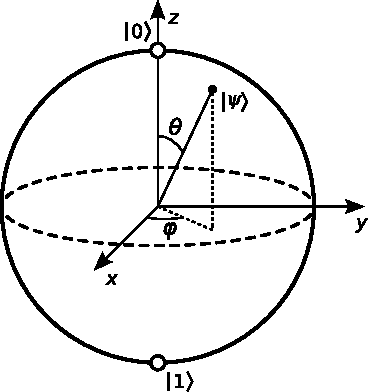
\includegraphics[width=.5\linewidth]{bloch}
				\caption{A single \emph{qubit} gate can be seen as a rotation on the Bloch Sphere}
			\end{figure}
		\end{minipage}
		\hfill
		\begin{minipage}{.48\linewidth}
			\begin{figure}
				\centering
				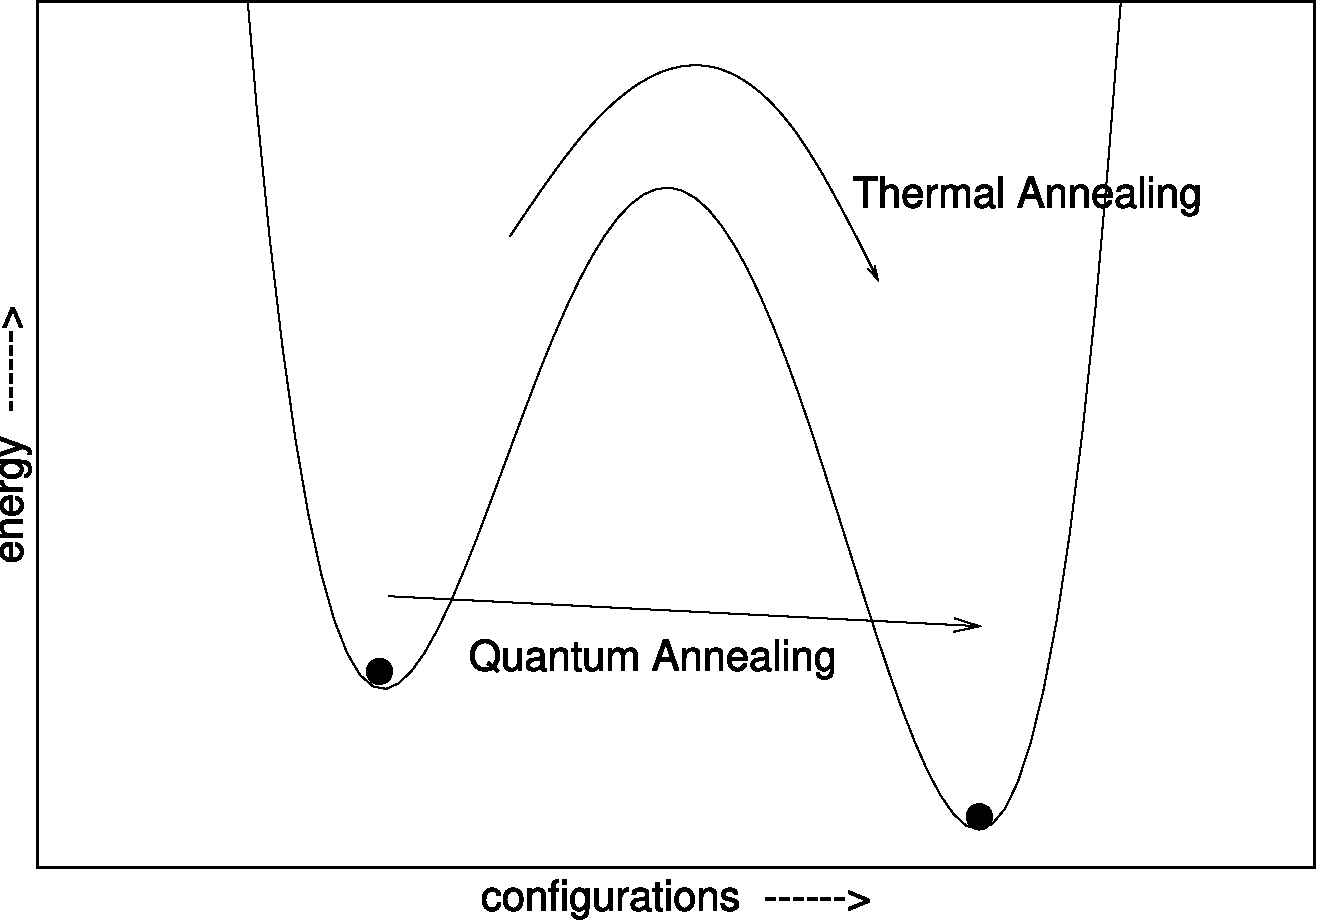
\includegraphics[width=.8\linewidth]{QA}
				\caption{Tunneling effect (K. Chakrabarti, A. Das)}
			\end{figure}
		\end{minipage}
	\end{minipage}
\end{frame}
	\section{QA-Prolog}
\begin{frame}{QA-Prolog}
	\begin{minipage}{.48\linewidth}
		\begin{block}{Il progetto}
			\begin{itemize}
				\item Sviluppato da Scott Pakin
				\item Python + GO
				\item Proof of concept
				\item Trasformazioni successive
				\item Prolog + Query $\rightarrow \mathcal{H}_f$  
				\item Interagisce direttamente con il solver
				\item Raccoglie e organizza i risultati
			\end{itemize}
		\end{block}
	\end{minipage}
	\hfill
	\begin{minipage}{.48\linewidth}
		\begin{figure}
			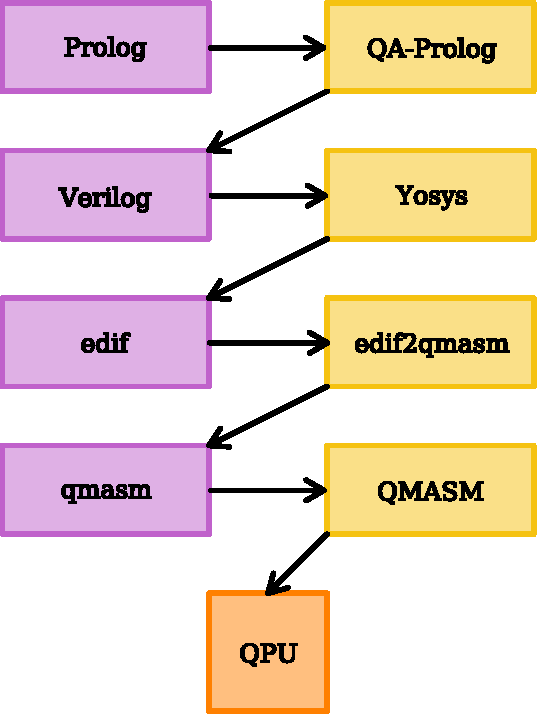
\includegraphics[width=.6\linewidth]{pipeline}
			\caption{Transformation pipeline}
		\end{figure}
	\end{minipage}
\end{frame}

\begin{frame}[fragile]{QMASM}{$\mathcal{H}_f$ simbolica  $\rightarrow$ $\mathcal{H}_f$ fisica}
	\begin{minipage}{.48\linewidth}
		\begin{block}{Cos'è}
			\begin{itemize}
				\item Quantum macro assembler
				\item Si interfaccia con Ocean
			\end{itemize}
		\end{block}
		\begin{block}{Cosa permette di fare}
			\begin{itemize}
				\item Riferimento simbolico a \emph{qubit}
				\item \emph{Qubit} \say{pinnati} a \texttt{TRUE} o \texttt{FALSE}
				\item Incapsulare pattern in macro
				\item Creazione di librerie di macro
				\item Organizzazione output
			\end{itemize}
		\end{block}
	\end{minipage}
	\hfill
	\begin{minipage}{.48\linewidth}
		\begin{figure}[h]
			\begin{minipage}{.6\linewidth}
				\hrule
				\begin{minted}{text}
					
# Y = A OR B
!begin_macro OR
$A  0.5
$B  0.5
$Y -1

$A $B  0.5
$A $Y -1
$B $Y -1
!end_macro OR
				\end{minted}
				\hrule
			\end{minipage}
			\caption{\textbf{or} gate}
		\end{figure}
		\vspace{-.5cm}
		\begin{center}
			\begin{minipage}{.8\linewidth}
				\begin{block}{}
					\centering
					Creiamo il file \texttt{gates.qmasm} 
				\end{block}
			\end{minipage}
		\end{center}
	\end{minipage}
\end{frame}

\begin{frame}[fragile]{QA-Prolog}
	\begin{minipage}{.42\linewidth}
		\begin{block}{}
			\begin{itemize}
				\item Traduzione da Prolog a Verilog
				\item Wrapper per tutta la Pipeline
				\item Risultati formato Human Readable
			\end{itemize}
		\end{block}
		\vspace{.3cm}
		\pause
		\[
		A \land \neg(B \lor C)
		\]
		\pause
		\begin{figure}[h]
			\begin{minipage}{.6\linewidth}
				\hrule
				\begin{minted}{Prolog}

sat(A, B, C, Y) :-
	or(B, C, X),
	not(X, Z),
	and(A, Z, Y).
				\end{minted}
				\hrule
			\end{minipage}
			\caption{Prolog Code}
		\end{figure}
	\end{minipage}
	\hfill
	\pause
	\begin{minipage}{.52\linewidth}
		\begin{figure}[h]
			\begin{minipage}{.9\linewidth}
				\hrule
				\begin{minted}{Verilog}
					
module sat (A, B, C, Y);
	input A, B, C;
	output Y;
	
	assign  Y = A & ~(B | C);
endmodule
				\end{minted}
				\hrule
			\end{minipage}
			\caption{Verilog Code}
		\end{figure}
		\pause
		\vspace{-.5cm}
		\begin{block}{Interrogazione}
			\begin{center}
				\scriptsize \texttt{QA-Prolog  --qmasm-args="--solver=tabu --postproc=opt" --query='sat(A, B, C, true).'  circ\_sat.pl}
			\end{center}
		\end{block}
		\begin{figure}
			\begin{minipage}{.4\linewidth}
				\hrule
				\begin{minted}{text}
					
			A = true
			B = false
			C = false
				\end{minted}
				\hrule
			\end{minipage}
			\caption{Query Result}
		\end{figure}
	\end{minipage}
\end{frame}

\begin{frame}[fragile]{QA-Prolog}{Esempio}
	\begin{minipage}{.48\linewidth}
		\begin{block}{Base di conoscenza}
			Il nemico del mio nemico è mio amico
		\end{block}
		\begin{figure}[h]
			\begin{minipage}{\linewidth}
				\hrule
				\begin{minted}{Prolog}
					
hates(alice, bob).
hates(bob, charlie).

enemies(P, Q) :- hates(P, Q).
enemies(P, Q) :- hates(Q, P).

friends(A, B) :-
	enemies(A, X),
	enemies(X, B),
	A \= B.
				\end{minted}
				\hrule
			\end{minipage}
			\caption{Enemy of my Enemy}
		\end{figure}
	\end{minipage}
	\hfill
	\pause
	\begin{minipage}{.48\linewidth}
		\begin{block}{Esecuzione}
			\begin{center}
				\scriptsize \texttt{QA-Prolog --qmasm-args="--postproc=opt" --query='friends(P1, P2).' friends.pl}
			\end{center}
		\end{block}
		\begin{figure}[h]
			\begin{minipage}{.3\linewidth}
				\hrule
				\begin{minted}{text}
					
	P1 = alice
	P2 = charlie
	
	P1 = charlie
	P2 = alice
				\end{minted}
				\hrule
			\end{minipage}
			\caption{Query Solution}
		\end{figure}
	\end{minipage}
\end{frame}
	\section{Ontology}
\begin{frame}{Ontologie}
		\begin{figure}
			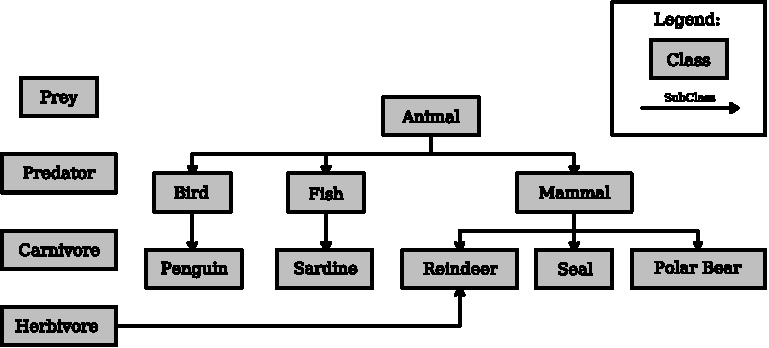
\includegraphics[width=.9\linewidth]{T-Box}
			\caption{Ontology T-Box}
		\end{figure}
\end{frame}


\begin{frame}[fragile]{Quantum Ontology}
	\begin{minipage}{.35\linewidth}
		\begin{block}{}
			\centering
			Traduzione in Prolog
		\end{block}
		\begin{figure}[h]
			\begin{minipage}{\linewidth}
				\hrule
				\begin{minted}{Prolog}

class(animal).
class(mammal).

subclass(mammal, animal).
subclass(seal, mammal).
				\end{minted}
				\hrule
			\end{minipage}
			\caption{Classes and subclasses}
		\end{figure}
\vspace{-.7cm}
		\begin{figure}[h]
			\begin{minipage}{\linewidth}
				\hrule
				\begin{minted}{Prolog}

subClass(C1, C2) :-
	subclass(C1, C2).
	
subClass(C1, C2) :-
	subclass(C1, C3),
	subClass(C3, C2).
				\end{minted}
				\hrule
			\end{minipage}
			\caption{Subclasses recursive definition}
		\end{figure}
	\end{minipage}
	\hfill
	\pause
	\begin{minipage}{.55\linewidth}
		\begin{block}{}
			\centering
			Unfolding
		\end{block}
		\begin{figure}[h]
			\hrule
			\begin{minipage}{.45\linewidth}
				\begin{minted}{Prolog}
					
subClass0(C0, C1) :-
	subclass(C0, C1).
	
subClass1(C0, C1) :-
	subClass0(C0, C2),
	subclass(C2, C1).
	
				\end{minted}
			\end{minipage}
			\hfill
			\begin{minipage}{.45\linewidth}
				\begin{minted}{Prolog}
subClass2(C0, C1) :-
	subClass1(C0, C2),
	subclass(C2, C1)
	
subClass3(C0, C1) :-
	subClass2(C0, C2),
	subclass(C2, C1)
				\end{minted}
			\end{minipage}
			\hrule
			\caption{Subclasses rule unfolded}
		\end{figure}
		\vspace{-.5cm}
		\begin{figure}[h]
			\begin{minipage}{\linewidth}
				\hrule
				\begin{minted}{Python}
					
rule_0 = 'subClass0(C0,C1) :- \n\tsubclass(C0, C1).\n'
for i in range(1, n_unfold):
	rule = 'subClass'+ str(i) + '(C0,C2) :-\n'        +\
		     '\tsubClass' + str(i-1) + '(C0,C3),\n'     +\
			   '\tsubclass(C3, C2).\n'
				\end{minted}
				\hrule
			\end{minipage}
			\caption{Unfolding script}
		\end{figure}
	\end{minipage}
\end{frame}

\begin{frame}[fragile]{Dimensione del problema}
	\hfill
		\begin{minipage}{.43\linewidth}
			\begin{block}{}
				\centering
				Query
			\end{block}
			\begin{figure}[h]
				\begin{minipage}{\linewidth}
					\hrule
					\begin{enumerate}
						\vspace{.1cm}
						\item \mintinline{Prolog}|?- class(animal).|\vspace{.1cm}
						\item \mintinline{Prolog}|?- class(X).|\vspace{.1cm}
						\item \mintinline{Prolog}|?- subClass(seal, X).|\vspace{.1cm}
						\item \mintinline{Prolog}|?- isA(sardy, X).|\vspace{.1cm}
						\item \mintinline{Prolog}|?- error(X, Y, Z).|\vspace{.1cm}
						\item \mintinline{Prolog}|?- hasProperty(I1, ancestor, reiny_c).|
					\end{enumerate}
					\hrule
				\end{minipage}
				\caption{Example Query}
			\end{figure}
		\end{minipage}
		\hfill
		\begin{minipage}{.48\linewidth}
			\begin{figure}
				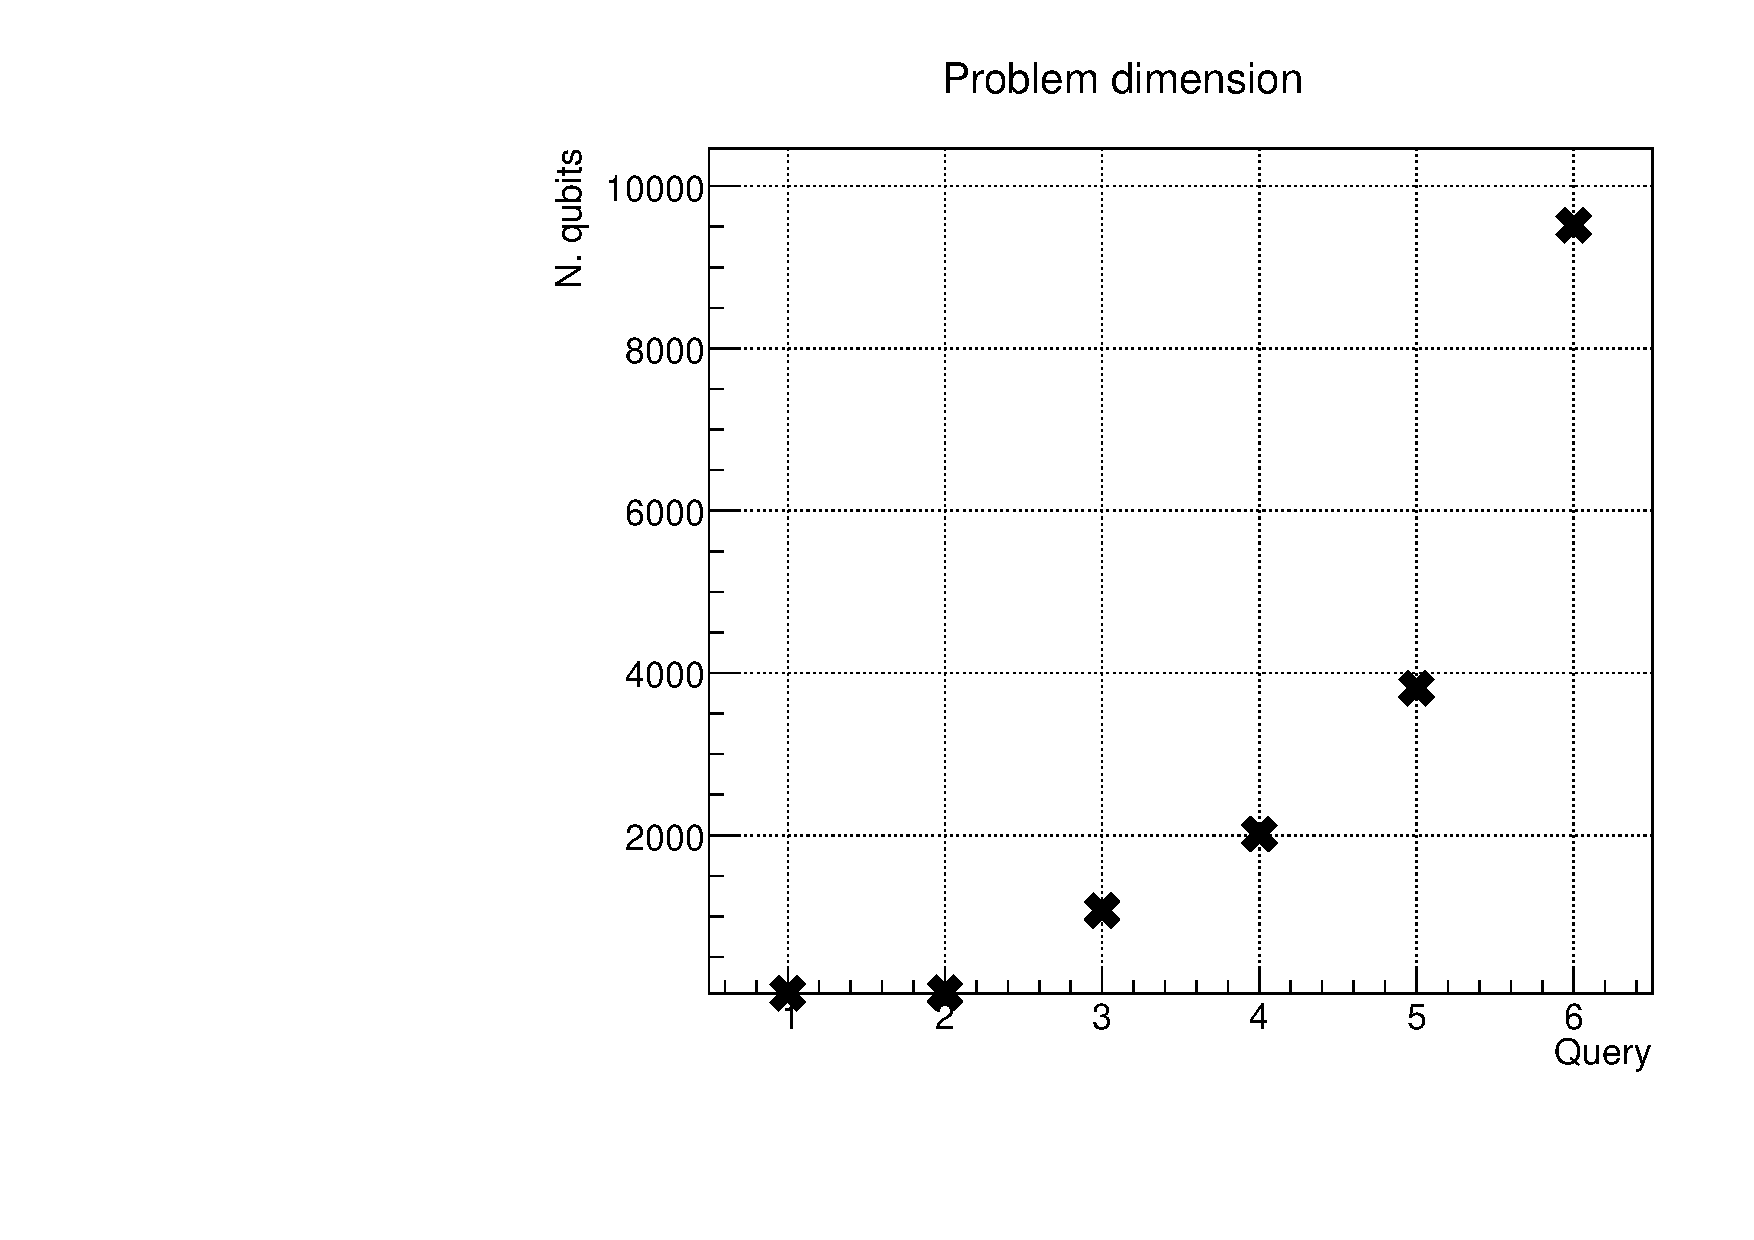
\includegraphics[width=.9\linewidth]{dimension}
				\caption{Problem Dimension}
			\end{figure}
		\end{minipage}
	\end{frame}

\begin{frame}[fragile]{Dimensione del problema}{Impatto dell'unfolding}
	\hfill
	\begin{minipage}{.4\linewidth}
		\begin{block}{}
			\centering
			Knowledge Base
		\end{block}
		\begin{figure}[h]
			\begin{minipage}{\linewidth}
				\hrule
				\begin{minted}{Prolog}
					
class(animal).
class(mammal).

subclass(mammal, animal).
				\end{minted}
				\hrule
			\end{minipage}
			\caption{Facts}
		\end{figure}
		\begin{figure}[h]
			\begin{minipage}{\linewidth}
				\hrule
				\begin{minted}{Prolog}
					
?- subClass(mammal, animal)
				\end{minted}
				\hrule
			\end{minipage}
			\caption{Query}
		\end{figure}
	\end{minipage}
	\hfill
	\begin{minipage}{.48\linewidth}
		\begin{figure}
			\includegraphics<1>[width=.9\linewidth]{unfold}
			\includegraphics<2>[width=.9\linewidth]{unfold_fit}
			\caption{Problem Dimension}
		\end{figure}
	\end{minipage}
\end{frame}
	\section{QAOA}
\begin{frame}{Non un solo paradigma}
	\begin{center}
		\begin{minipage}{.6\linewidth}
			\begin{block}{}
				\centering
				Problema QUBO/Ising
				\vspace{-.3cm}
				\[
				\mathcal{H}_f
				\]
			\end{block}
		\end{minipage}
	\end{center}
	\begin{figure}[h]
		\centering
		\begin{subfigure}{0.3\linewidth}
			\centering
			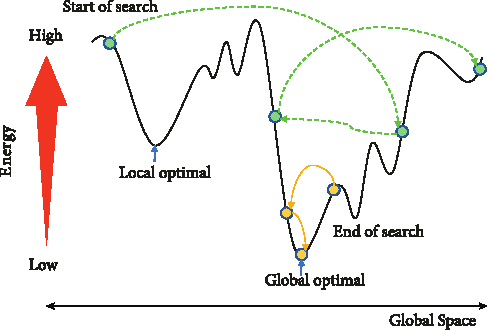
\includegraphics[width=\linewidth]{simulate_annealing}
			\caption{Simulated annealing (Li Yang)}
		\end{subfigure}
		\hfill
		\begin{subfigure}{0.3\linewidth}
			\centering
			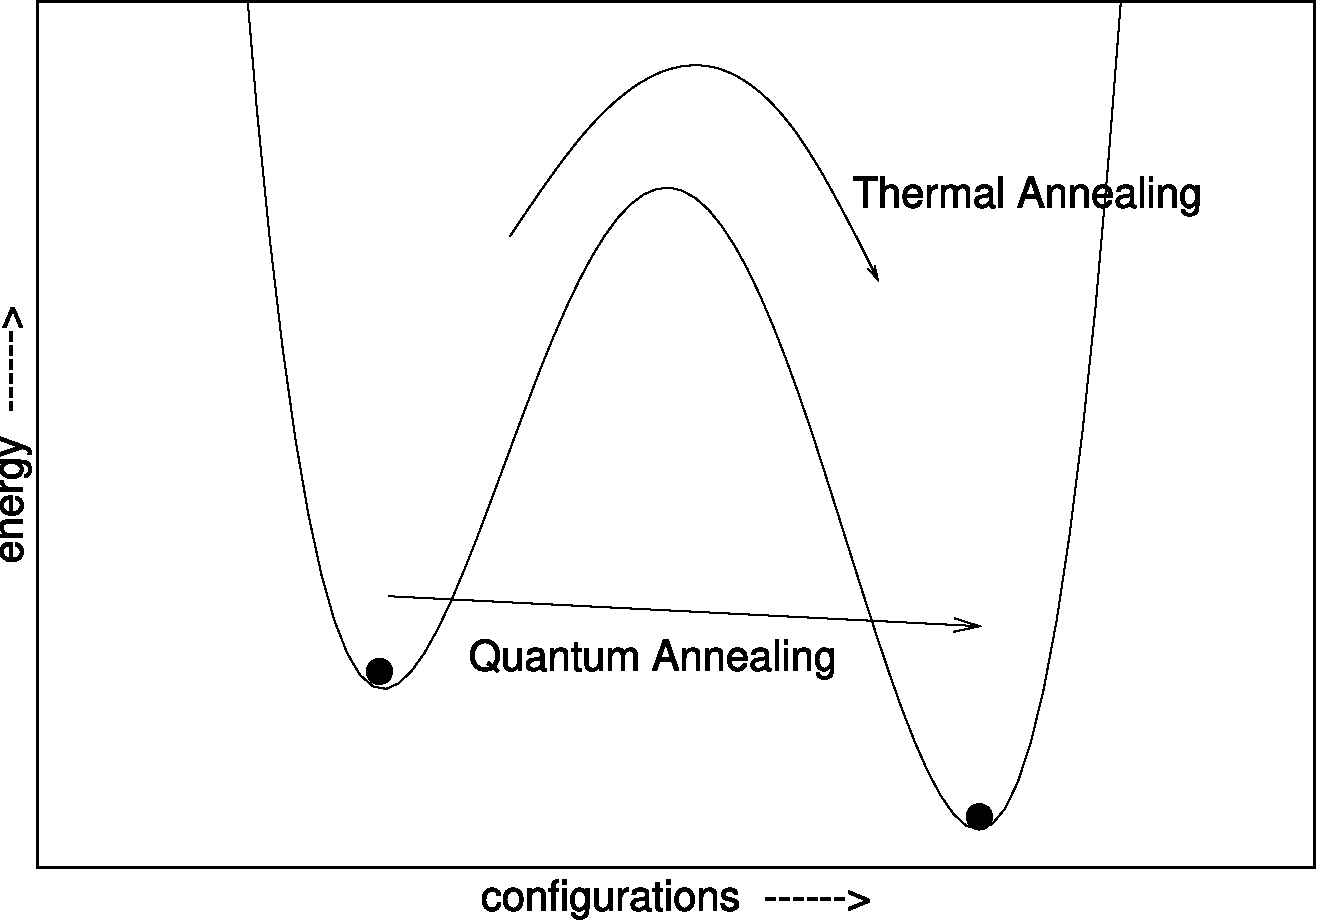
\includegraphics[width=\linewidth]{QA}
			\caption{Quantum annealing (K. Chakrabarti, A. Das)}
		\end{subfigure}
		\hfill
		\begin{subfigure}{0.3\linewidth}
			\centering
			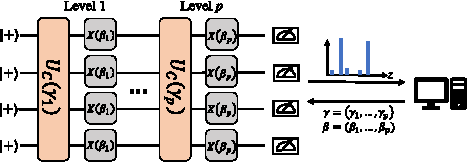
\includegraphics[width=\linewidth]{QAOA_sketch}
			\caption{QAOA (Z. Zhou, Y. Du, X. Tian, D. Tao)}
		\end{subfigure}
		\caption{Single rappresentation 3 different approaches}
	\end{figure}
\end{frame}

\begin{frame}[fragile]{Esempio}
	\begin{minipage}{.33\linewidth}
		\begin{figure}[h]
			\vspace{.3cm}
			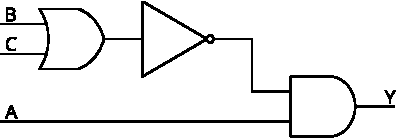
\includegraphics[width=.8\linewidth]{sat_circ.pdf}
			\vspace{.5cm}
			\hrule
			\begin{minted}{text}
				
				!begin_macro sat
				!use_macro AND $id00006
				!use_macro NOT $id00004
				!use_macro OR $id00005
				$id00004.A = $id00005.Y
				$id00005.A = b
				$id00005.B = c
				$id00006.A = a
				$id00006.B = $id00004.Y
				$id00006.Y = y
				!end_macro sat
			\end{minted}
			\hrule
			\caption{CircSat}
		\end{figure}
	\end{minipage}
	\hfill
	\begin{minipage}{.65\linewidth}
		{
			\tiny
			\[
			\begin{pmatrix}
				0.5 & 0.5 & -1 & 0 & 0 & 0 & 0 & 0 & 0 & 0 & -2 \\
				0 & 0.5 & -1 & 0 & -2 & 0 & 0 & 0 & 0 & 0 & 0 \\
				0 & 0 & 1 & 0 & 0 & 0 & 0 & 0 & 0 & 0 & 0 \\
				0 & 0 & 0 & 0 & 1 & 0 & 0 & -2 & 0 & 0 & 0 \\
				0 & 0 & 0 & 0 & 0 & 0 & 0 & 0 & 0 & 0 & 0 \\
				0 & 0 & 0 & 0 & 0 & -0.5 & 0.5 & -1 & -2 & 0 & 0 \\
				0 & 0 & 0 & 0 & 0 & 0 & -0.5 & -1 & 0 & -2 & 0 \\
				0 & 0 & 0 & 0 & 0 & 0 & 0 & 1 & 0 & 0 & 0 \\
				0 & 0 & 0 & 0 & 0 & 0 & 0 & 0 & 0 & 0 & 0 \\
				0 & 0 & 0 & 0 & 0 & 0 & 0 & 0 & 0 & 0 & 0 \\
				0 & 0 & 0 & 0 & 0 & 0 & 0 & 0 & 0 & 0 & 0
			\end{pmatrix}
			\]
		}
		\vspace{-.4cm}
		\begin{figure}[h]
			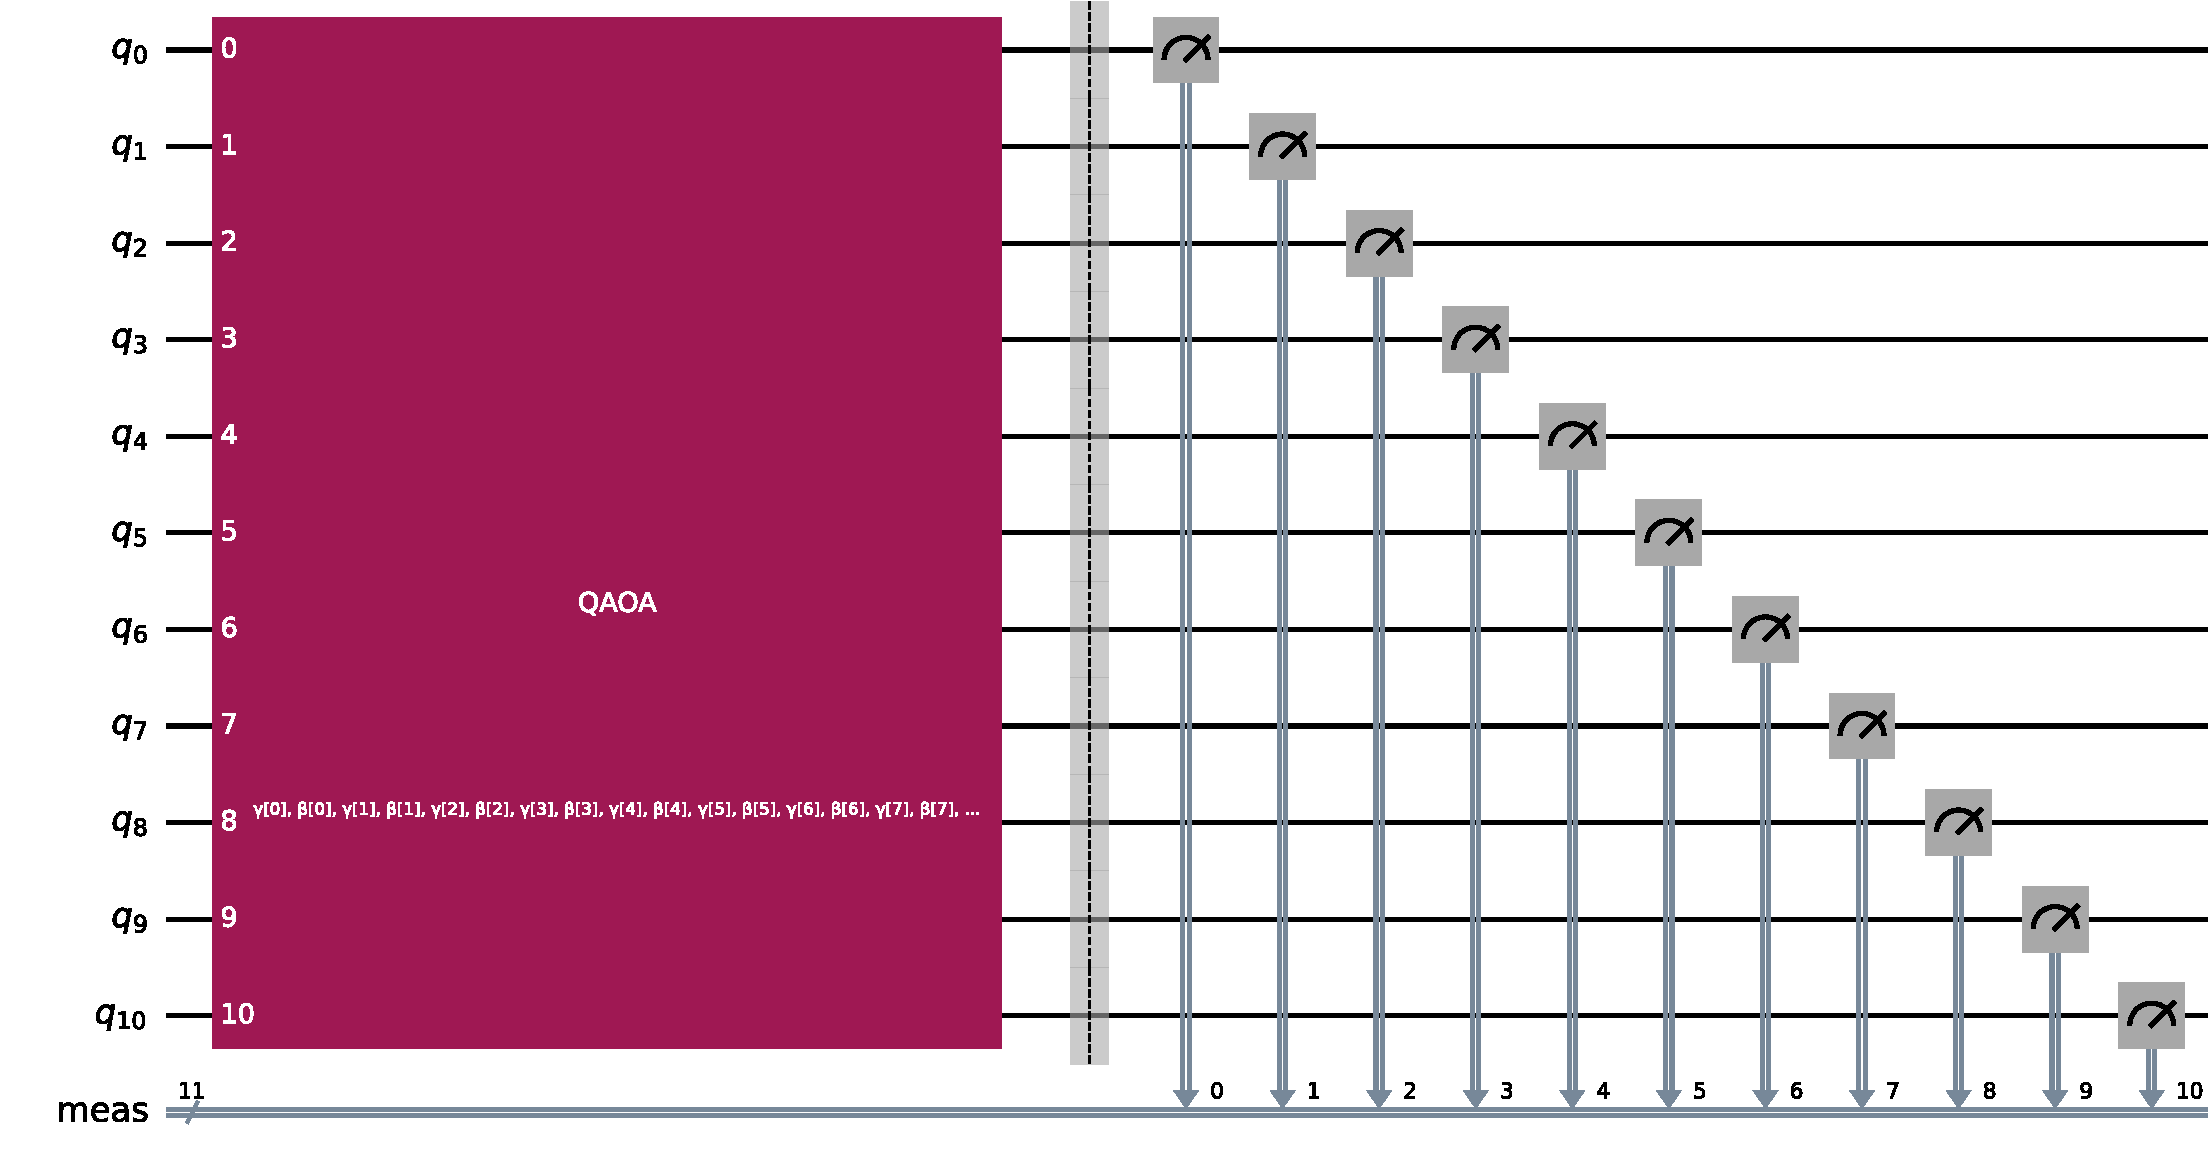
\includegraphics[width=.65\linewidth]{QAOA_qc}
			\vspace{-.1cm}
			\caption{$\mathcal{H}_f$ and QAOA Quantum Circuit}
		\end{figure}
	\end{minipage}
\end{frame}

\begin{frame}{Esempio}{Risultato}
	\begin{minipage}{.337\linewidth}
		\begin{figure}
			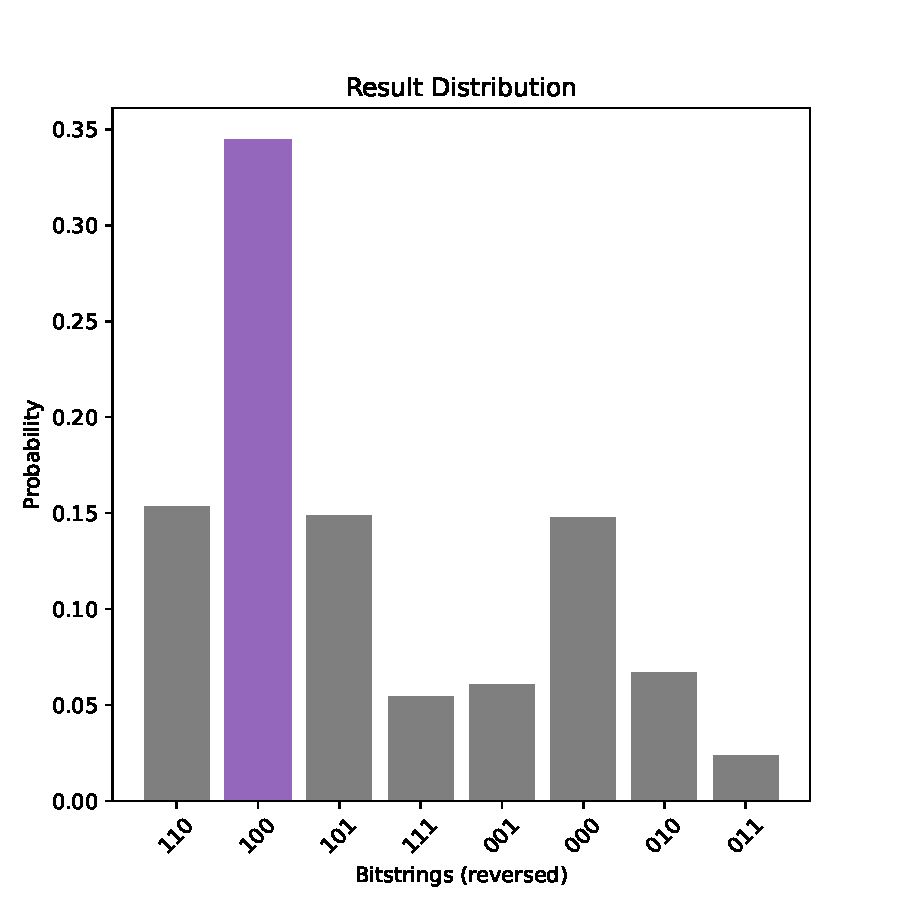
\includegraphics[width=\linewidth]{QAOA_r_2}
			\caption{3 \say{interesting} bit}
		\end{figure}
	\end{minipage}
	\hfill
	\begin{minipage}{.65\linewidth}
		\begin{figure}
			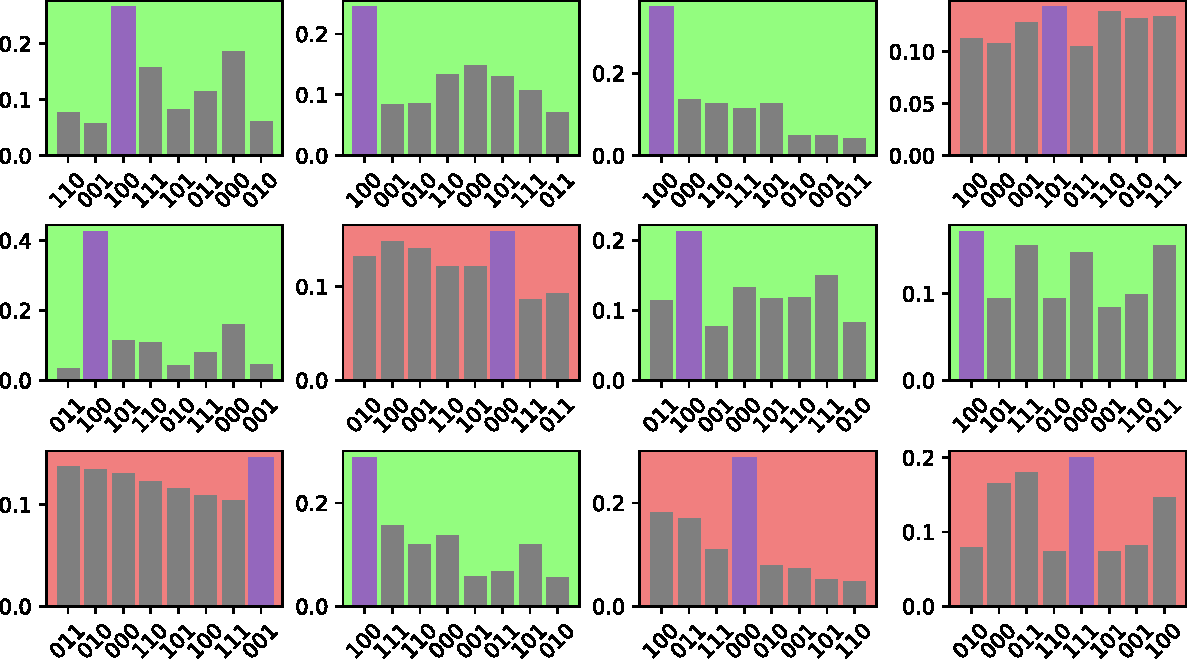
\includegraphics[width=\linewidth]{QAOA_r_3}
			\caption{Multilpe experiment runs}
		\end{figure}
	\end{minipage}
\end{frame}
	\section{Lavoro Futuro}
\begin{frame}{Lavoro Futuro}
	\begin{minipage}{.45\linewidth}
		\begin{block}{Monte}
			\begin{itemize}
				\item Compilatore Ontologie $\rightarrow$ KB Prolog
			\end{itemize}
		\end{block}
	\end{minipage}
	\hfill
	\begin{minipage}{.45\linewidth}
		\begin{block}{Valle}
			\begin{itemize}
				\item Interfacciare QMASM con altri solver
			\end{itemize}
		\end{block}
	\end{minipage}
	\vspace{.5cm}
	\begin{center}
		\begin{minipage}{.7\linewidth}
			\begin{block}{}
				\begin{itemize}
					\item Mantenere aggiornati i componenti \only<2>{(metà del lavoro di tesi)}
					\item Testare su hardware quantistico
					\item Confronto QA e QAOA
				\end{itemize}
			\end{block}
		\end{minipage}
	\end{center}
\end{frame}
	\part{Ringraziamenti}
	\begin{frame}[plain]
		{
			\Huge
			Grazie per l'attenzione \only<2>{\Large Domande?} \hfill 
\includegraphics[width=.06\linewidth]{logo_col_small}
		}
		\centering
		\includegraphics[width=\linewidth]{fine}\\
\end{frame}
	\setcounter{framenumberbeforeappendix}{\value{framenumber}}
	\part{Materiale aggiuntivo}
	\section{Appendici}
\begin{frame}{Perché il quantum computing}
	\begin{minipage}{\linewidth}
		\begin{minipage}{.3\linewidth}
			\begin{block}{Grazie a}
				\begin{itemize}
					\item Superposition
					\item Entanglement
				\end{itemize}
			\end{block}
		\end{minipage}
		\hfill
		\begin{minipage}{.68\linewidth}
			\begin{gather*}
				\mathcal{H}(t) \Ket{\psi(t)} = i \hbar \frac{\partial}{\partial t} \Ket{\psi(t)}\\ 
				\Braket{A_0 \otimes B_0} + \Braket{A_0 \otimes B_1} + \Braket{A_1 \otimes B_0} - \Braket{A_1 \otimes B_1} = 2\sqrt{2}
			\end{gather*}
		\end{minipage}
	\end{minipage}
	\begin{minipage}{\linewidth}
		\begin{minipage}{.3\linewidth}
			\begin{block}{Violiamo}
				\begin{center}
					Strong Church-Turing Thesis
				\end{center}
			\end{block}
		\end{minipage}
		\hfill
		\begin{minipage}{.68\linewidth}
			\vspace{.5cm}
			\begin{figure}
				\centering
				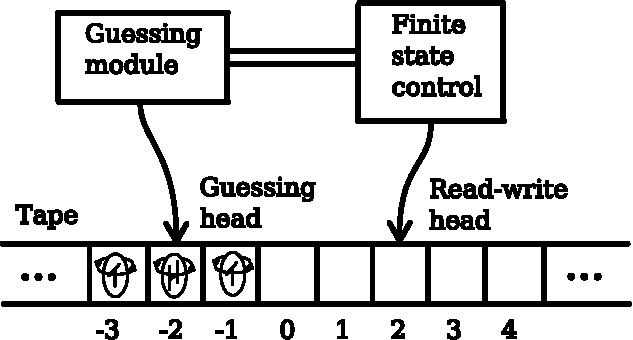
\includegraphics[width=.6\linewidth]{ntm}
				\caption{Probabilistic Turing Machine}
			\end{figure}
		\end{minipage}
	\end{minipage}
\end{frame}

\begin{frame}{Quantum Gate}
	\begin{minipage}{.35\linewidth}
		\begin{block}{}
			\begin{itemize}
				\item Formalismo molto studiato
				\item Gate Reversibili
				\item  Set di porte universali
				\item  Algoritmi di Shore, ecc.
			\end{itemize}
		\end{block}
	\end{minipage}
	\hfill
	\begin{minipage}{.6\linewidth}
		\begin{figure}
			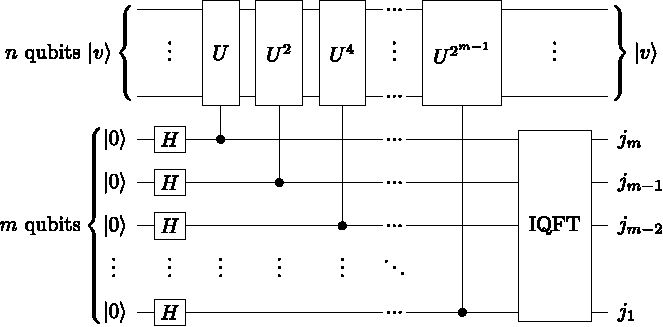
\includegraphics[width=\linewidth]{Shor}
			\caption{Step for Shor algoritm (Thomas G. Wong)}
		\end{figure}
	\end{minipage}
\end{frame}


\begin{frame}{Quantum Annealer}
	\begin{minipage}{.48\linewidth}
		\begin{figure}
			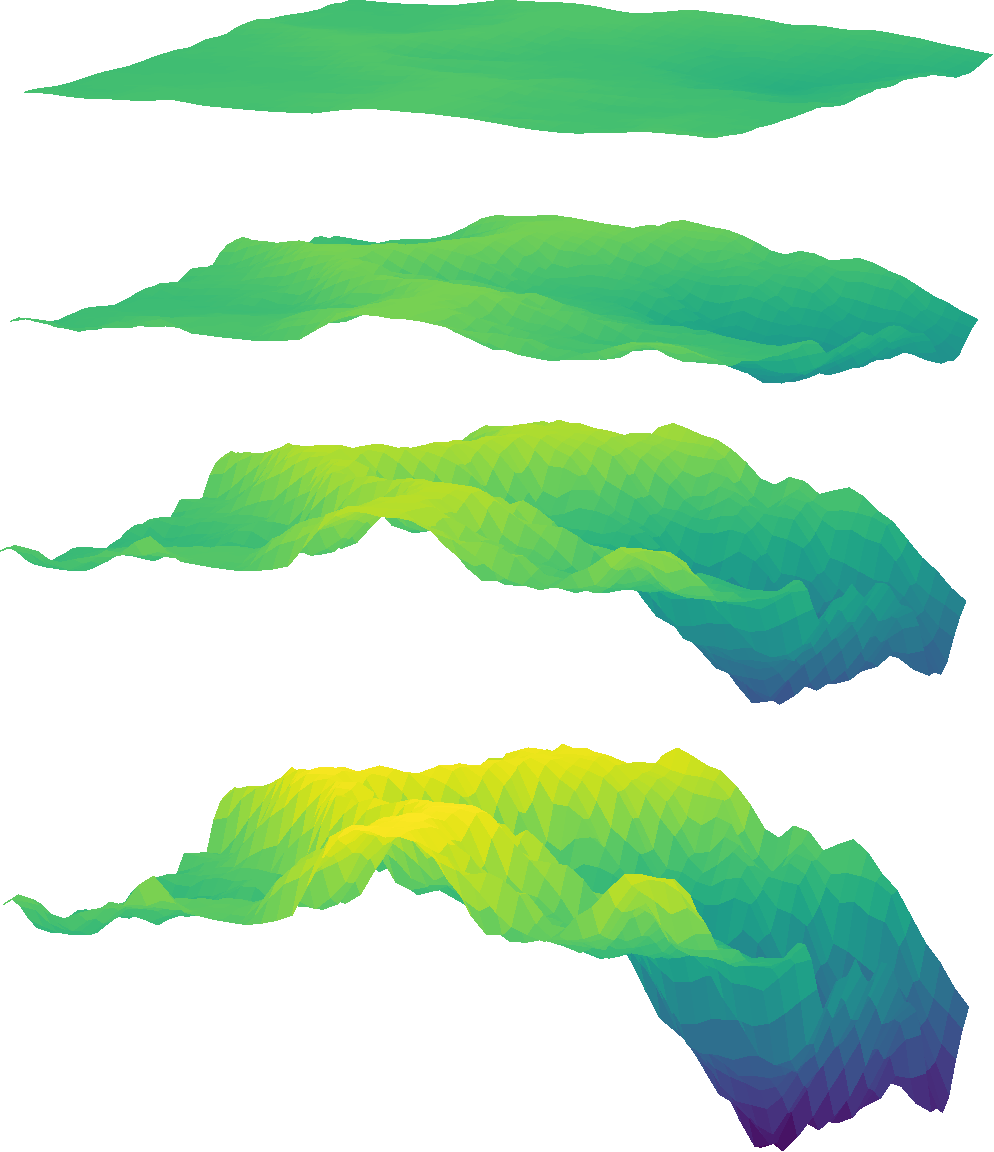
\includegraphics[width=.65\linewidth]{QA_fun}
			\caption{Complete sovrapposition $\rightarrow$ ground state $\mathcal{H}_f$}
		\end{figure}
	\end{minipage}
	\hfill
	\begin{minipage}{.48\linewidth}
		\begin{block}{}
			\begin{itemize}
				\item Problemi in forma QUBO
				\item Ispirato a Simulated Annealling
				\item Effetto tunneling
				\item Adiabatic Quantum Computing (AQC)
				\item $\mathcal{H}(t) =s(t) \mathcal{H}_i + (i-s(t)) \mathcal{H}_f $
			\end{itemize}
		\end{block}
	\end{minipage}	
\end{frame}

\begin{frame}[fragile]{QMASM}{Esempio: Macro}
	\begin{minipage}{.3\linewidth}
		\begin{figure}[h]
			\begin{minipage}{\linewidth}
				\hrule
				\begin{minted}{text}
					
# Y = A OR B
!begin_macro OR
	$A  0.5
	$B  0.5
	$Y -1
	
	$A $B  0.5
	$A $Y -1
	$B $Y -1
!end_macro OR
				\end{minted}
				\hrule
			\end{minipage}
			\caption{\textbf{or} gate}
		\end{figure}
	\end{minipage}
	\hfill
	\begin{minipage}{.3\linewidth}
		\begin{figure}[h]
			\begin{minipage}{\linewidth}
				\hrule
				\begin{minted}{text}
					
# Y = NOT A
	!begin_macro NOT
	$A $Y 1.0
!end_macro NOT
				\end{minted}
				\hrule
			\end{minipage}
			\caption{\textbf{not} gate}
		\end{figure}
	\end{minipage}
	\hfill
	\begin{minipage}{.3\linewidth}
		\begin{figure}[h]
			\begin{minipage}{\linewidth}
				\hrule
				\begin{minted}{text}

# Y = A AND B
!begin_macro AND
	$A -0.5
	$B -0.5
	$Y  1
	
	$A $B  0.5
	$A $Y -1
	$B $Y -1
!end_macro AND
				\end{minted}
				\hrule
			\end{minipage}
			\caption{\textbf{and} gate}
		\end{figure}
	\end{minipage}
	\begin{block}{}
		\centering
		possiamo racchiudere queste macro nel file \texttt{gates.qmasm}
	\end{block}
\end{frame}

\begin{frame}[fragile]{QMASM}{Esempio: $y = x_1 \land \neg(x_2 \lor x_3)$}
	\begin{center}
		\begin{minipage}{.25\linewidth}
			\begin{figure}[h]
				\begin{minipage}{\linewidth}
					\hrule
					\begin{minted}{text}
						
!include <gates>

!use_macro OR x2_or_x3
	x2_or_x3.$A = x2
	x2_or_x3.$B = x3
	x2_or_x3.$Y = $x4

!use_macro NOT not_x4
	not_x4.$A = $x4
	not_x4.$Y = $x5

!use_macro AND x1_and_x5
	x1_and_x5.$A = x1
	x1_and_x5.$B = $x5
	x1_and_x5.$Y = y
					\end{minted}
					\hrule
				\end{minipage}
				\caption{CircSat problem}
			\end{figure}
		\end{minipage}
		\hspace{1cm}
		\begin{minipage}{.6\linewidth}
			\begin{block}{}
				\say{Pinniamo} il valore di $y$ per ottenere l'assegnamento delle $x_i$ che verificano la formula logica:
				\begin{center}
					\scriptsize \texttt{qmasm --run --pin="y := true" circsat.qmasm}
				\end{center}
			\end{block}
			\begin{figure}[h]
				\centering
				\begin{minipage}{.72\linewidth}
					\hrule
					\begin{minted}{text}
						
Solution #1 (energy = -20.0000, tally = 647):

							Variable  Value
							--------  -----
							x1        True
							x2        False
							x3        False
							y         True
					\end{minted}
					\hrule
				\end{minipage}
				\caption{CircSat solution}
			\end{figure}
		\end{minipage}
	\end{center}
\end{frame}

\begin{frame}[fragile]{Yosys - edif2qmasm}{Esempio: moltiplicazione tra interi}
	\begin{minipage}{.48\linewidth}
		\begin{figure}[h]
			\begin{minipage}{\linewidth}
				\hrule
				\begin{minted}{Verilog}
					
module mult (multiplicand, multiplier, product);
	input [1:0] multiplicand;
	input [1:0] multiplier;
	output[2:0] product;
	
	assign product = multiplicand * multiplier;
endmodule
				\end{minted}
				\hrule
			\end{minipage}
			\caption{Factorization problem}
		\end{figure}
		\vspace{-.7cm}
		\begin{block}{Traduzione in EDIF}
			\begin{center}
				\scriptsize \texttt{yosys myfile.v synth.ys -b edif -o myfile.edif}
			\end{center}
		\end{block}
		\begin{block}{Traduzione in QMASM}
			\begin{center}
				\scriptsize \texttt{edif2qmasm -o="myfile.qmasm" myfile.edif}
			\end{center}
		\end{block}
	\end{minipage}
	\hfill
	\begin{minipage}{.48\linewidth}
		\begin{block}{Esecuzione}
			\begin{center}
				\scriptsize \texttt{qmasm --run --pin="mult.product[2:0] := 110" --solver="sim\_anneal" mult.qmasm}
			\end{center}
		\end{block}
		\vspace{-.1cm}
		\begin{figure}[h]
			\begin{minipage}{.9\linewidth}
				\hrule
				\begin{minted}{text}
					
Solution #1 (energy = -57.5000, tally = 68):

				Variable              Value
				--------------------  -----
				mult.multiplicand[0]  False
				mult.multiplicand[1]  True
				mult.multiplier[0]    True
				mult.multiplier[1]    True
				mult.product[0]       False
				mult.product[1]       True
				mult.product[2]       True
				\end{minted}
				\hrule
			\end{minipage}
			\caption{Factorization Solution}
		\end{figure}
	\end{minipage}
\end{frame}

\begin{frame}[fragile]{Update al progetto}{Incompatibilità tra output edif2qmasm e input QMASM}
	\begin{minipage}{.31\linewidth}
		\begin{figure}
			\begin{minipage}{.95\linewidth}
				\hrule
				\begin{minted}{verilog}
					
// Define hates(atom, atom).
module \hates/2 (A, B, Valid);
	...
endmodule
				\end{minted}
				\hrule
			\end{minipage}
			\caption{Verilog}
		\end{figure}
		\vspace{-.6cm}
		\begin{figure}
			\begin{minipage}{.95\linewidth}
				\hrule
				\begin{minted}{text}
					
# hates/2
!begin_macro id00011
	...
!end_macro id00011

# enemies/2
!begin_macro id00010
!use_macro OR $id00031
!use_macro hates/2
...
				\end{minted}
				\hrule
				\caption{qmasm}
			\end{minipage}
		\end{figure}
	\end{minipage}
	\hfill
	\begin{minipage}{.67\linewidth}
		\begin{figure}
			\begin{minipage}{.95\linewidth}
				\hrule
				\begin{minted}{python}
					
with open(file, 'r') as input:
first = input.readline()
second = input.readline()
while(second_row != ""):
	if first.startswith("#") and second.startswith("!begin_macro"):
		self.name[first[2:-1]] = second[len("!begin_macro "):-1]
	first_row = second_row
	second_row = input.readline()

with open(file, 'r') as input:
doc = input.read()
lines = doc.splitlines()
for line in lines:
	for word in line.split():
		if word in self.name.keys():
			line = line.replace(word, self.name[word])
	self.new_lines.append(line)
				\end{minted}
				\hrule
			\end{minipage}
			\caption{Preprocessing}
		\end{figure}
	\end{minipage}
\end{frame}

\begin{frame}{Ontologie}
	\begin{minipage}{.48\linewidth}
		\begin{block}{Cos'è un'ontologia}
			\begin{itemize}
				\item Insieme di fatti
				\item Riguardanti un dominio di interesse
				\item Prevengono interpretazioni sbagliate
				\item Assicurano la cooperazione tra software
			\end{itemize}
		\end{block}
		\begin{block}{Come si definisce un'ontologia}
			\begin{itemize}
				\item Ontology Web Language (OWL)
				\item Diversi \say{flavours}
				\begin{itemize}
					\item OWL Full
					\item OWL DL
				\end{itemize}
				\item Classi Individui e Relazioni
			\end{itemize}
		\end{block}
	\end{minipage}
	\hfill
	\begin{minipage}{.48\linewidth}
		\begin{figure}[h]
			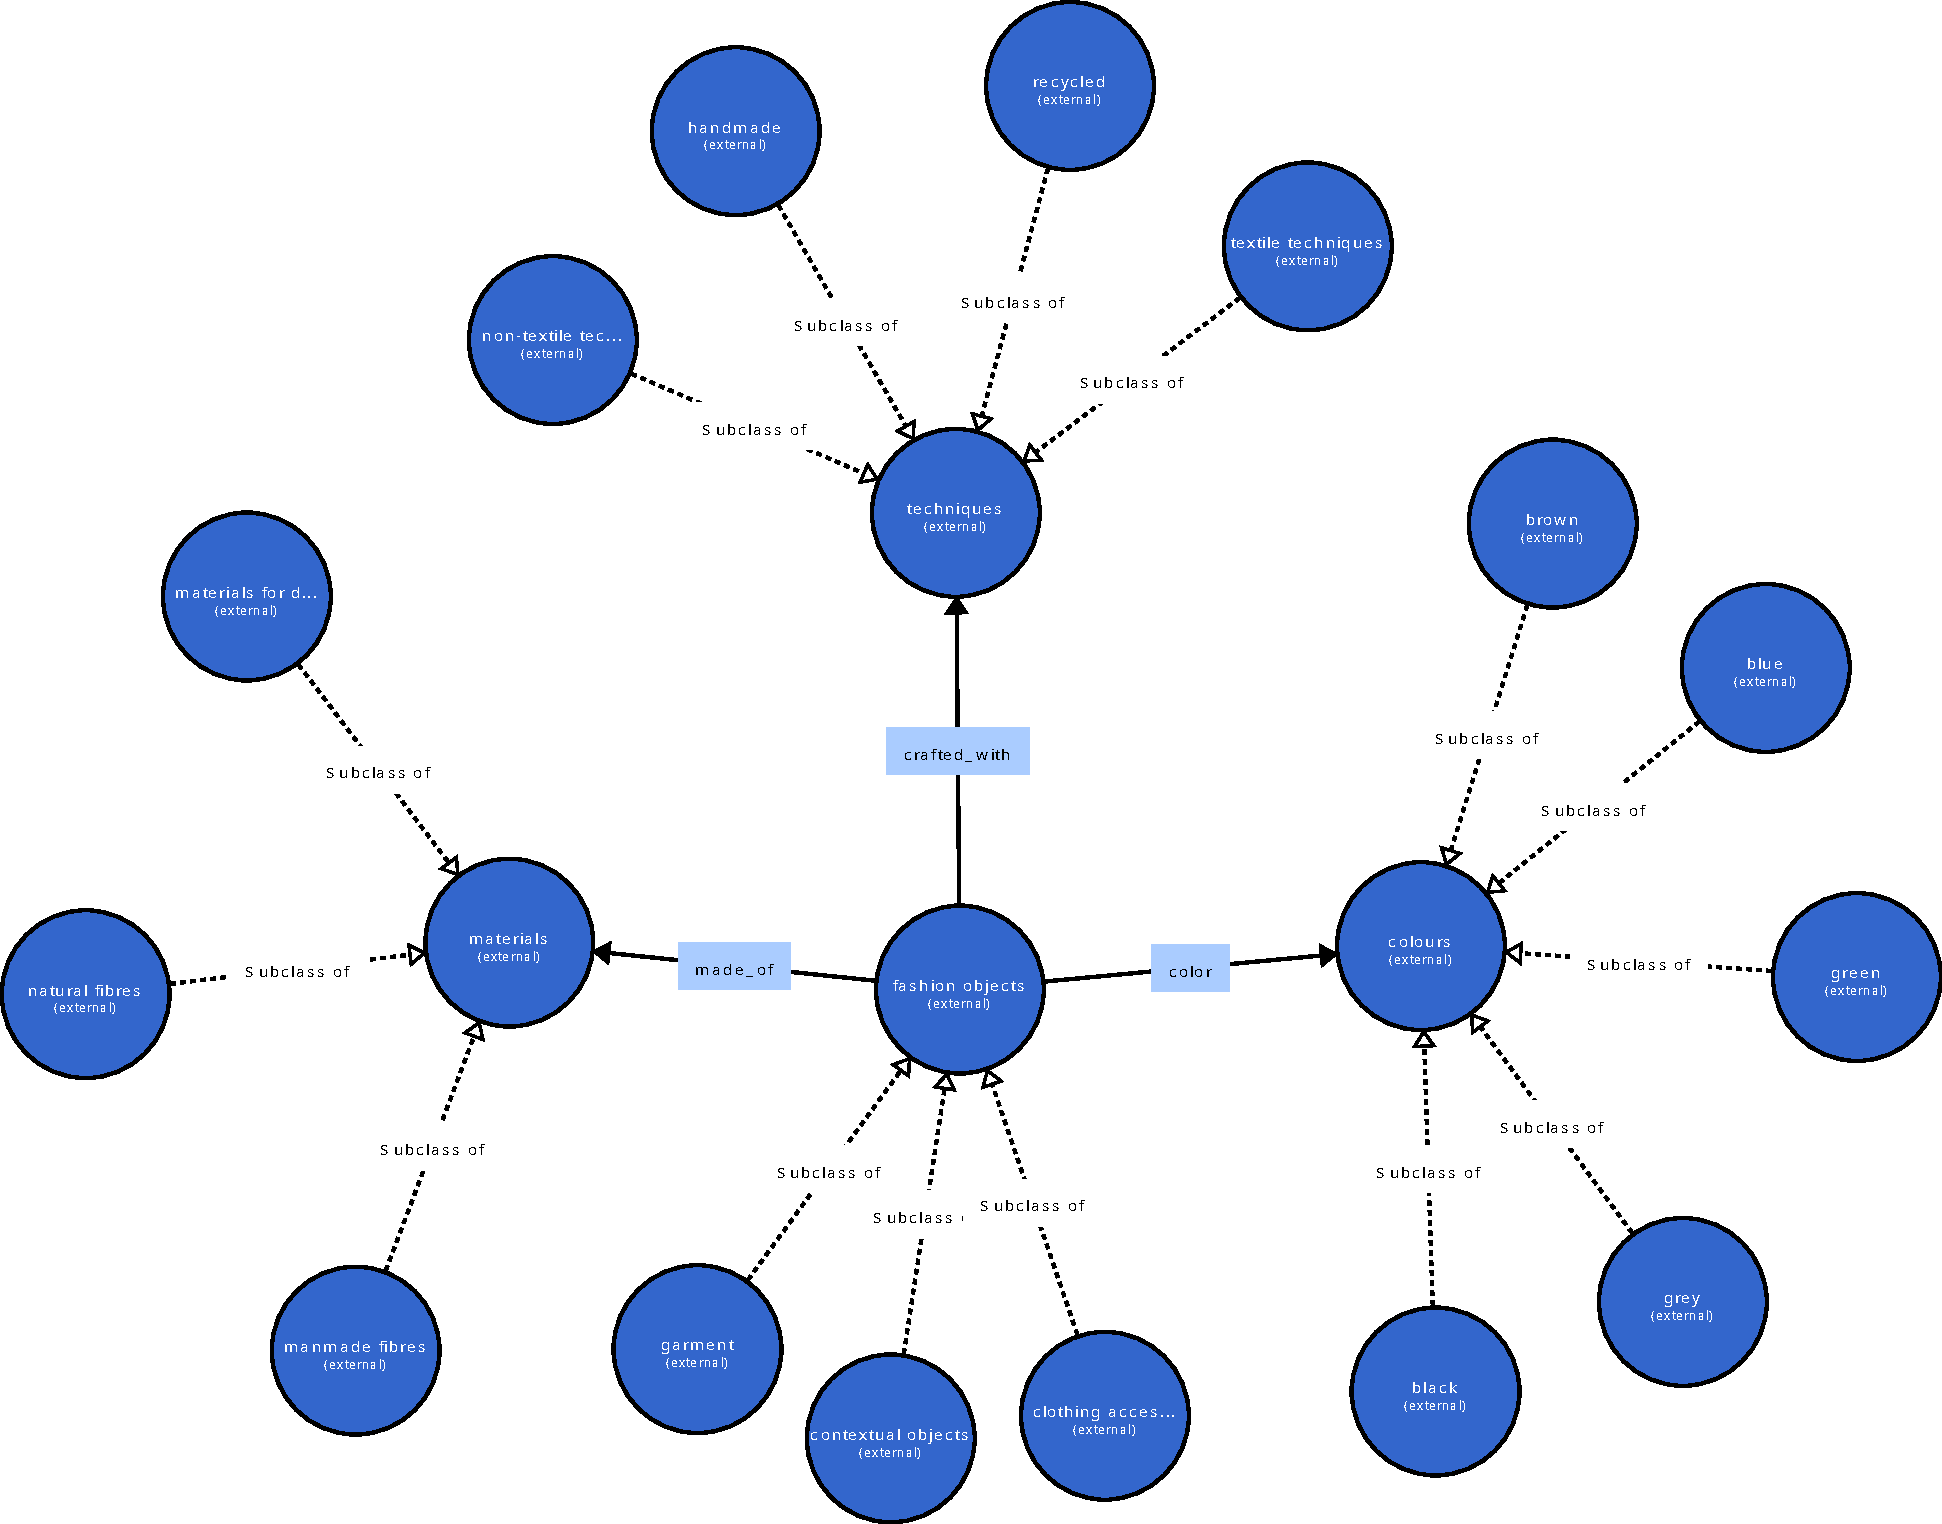
\includegraphics[width=\linewidth]{europeana_relation.pdf}
		\end{figure}
	\end{minipage}
\end{frame}

\begin{frame}{Inferenze in OWL}
	\begin{minipage}{.48\linewidth}
		\begin{block}{Complessità}
			\begin{itemize}
				\item Variazione sintattica di $\mathcal{SROIQ}$
				\item $\mathcal{ALC}$ è una restrizione di $\mathcal{SROIQ}$
				\item $\mathcal{ALC}$ è PSpace-hard
			\end{itemize}
		\end{block}
		\begin{block}{Reasoner}
			\begin{itemize}
				\item Pellet
				\item Fact++
				\item HermiT
				\item \dots
			\end{itemize}
		\end{block}
	\end{minipage}
	\hfill
	\begin{minipage}{.48\linewidth}
		\begin{figure}[h]
			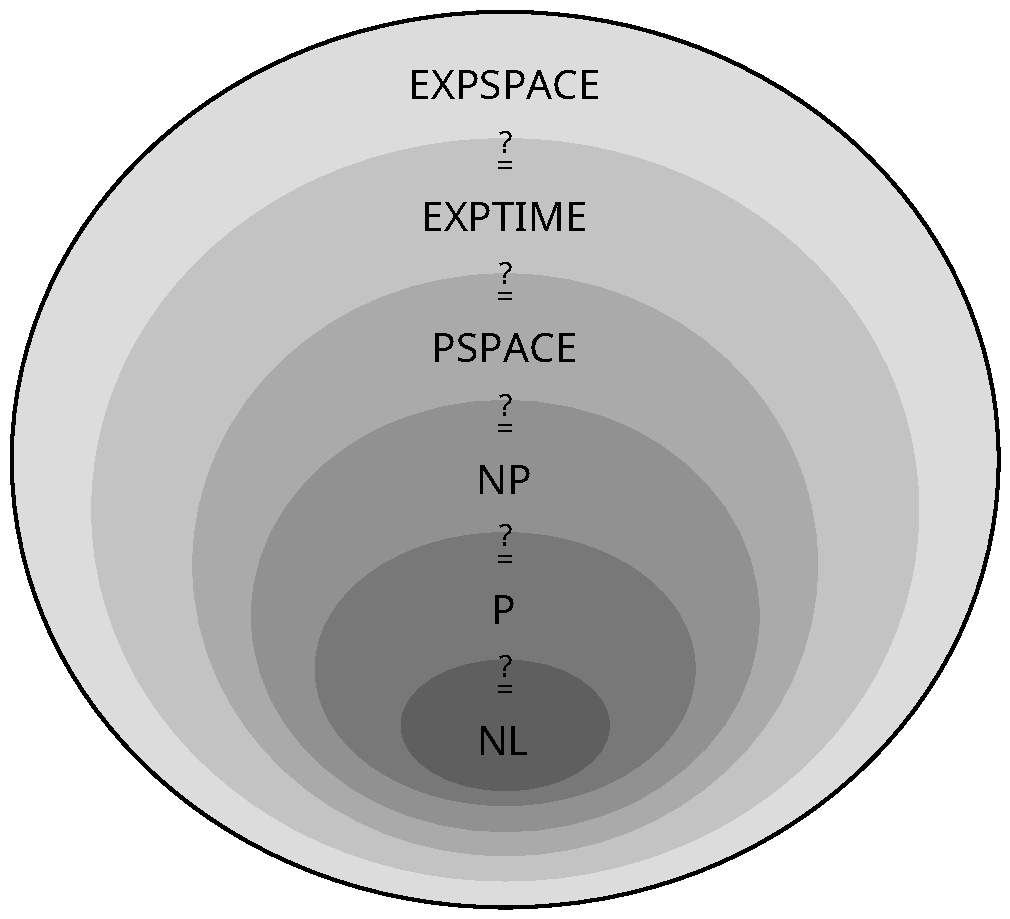
\includegraphics[width=.8\linewidth]{Complexity.pdf}
		\end{figure}
	\end{minipage}
\end{frame}
	\setcounter{framenumber}{\value{framenumberbeforeappendix}}
\end{document}